\documentclass{sigchi-ext}
% Please be sure that you have the dependencies (i.e., additional LaTeX packages) to compile this example.
% See http://personales.upv.es/luileito/chiext/

\copyrightinfo{
  Permission to make digital or hard copies of all or part of this work for
  personal or classroom use is granted without fee provided that copies are
  not made or distributed for profit or commercial advantage and that
  copies bear this notice and the full citation on the first page. To copy
  otherwise, or republish, to post on servers or to redistribute to lists,
  requires prior specific permission and/or a fee.\\
  \emph{CHI'12}, May 5--10, 2012, Austin, Texas, USA.\\
  Copyright 2012 ACM 978-1-4503-1016-1/12/05...\$10.00.\\
}

\title{Wordcraft: Playing with Sentence Structure}

\numberofauthors{7}
% Notice how author names are alternately typesetted to appear ordered in 2-column format;
% i.e., the first 4 autors on the first column and the other 4 auhors on the second column.
% Actually, it's up to you to strictly adhere to this author notation.
\author{
  \vspace{4em} % lisatolles: The abstract heading should start at the same height as the authors names
  \alignauthor{
  	\textbf{First Author}\\
  	\affaddr{AuthorCo, Inc.}\\
%  	\affaddr{123 Author Ave.}\\
  	\affaddr{Authortown, PA 54321 USA}\\
  	\email{author1@anotherco.com}
  }\alignauthor{
  	\textbf{Fourth Author}\\
  	\affaddr{AuthorCo, Inc.}\\
%  	\affaddr{123 Author Ave.}\\
  	\affaddr{Authortown, PA 54321 USA}\\
  	\email{author4@anotherco.com}
  }\vfil
  \alignauthor{
  	\textbf{Second Author}\\
  	\affaddr{AuthorCo, Inc.}\\
%  	\affaddr{123 Author Ave.}\\
  	\affaddr{Authortown, PA 54321 USA}\\
  	\email{author2@anotherco.com}
  }\alignauthor{
  	\textbf{Fifth Author}\\
  	\affaddr{AuthorCo, Inc.}\\
%  	\affaddr{123 Author Ave.}\\
  	\affaddr{Authortown, PA 54321 USA}\\
  	\email{author5@anotherco.com}
  }\vfil
  \alignauthor{
  	\textbf{Third Author}\\
  	\affaddr{AuthorCo, Inc.}\\
%  	\affaddr{123 Author Ave.}\\
  	\affaddr{Authortown, PA 54321 USA}\\
  	\email{author3@anotherco.com}
  }\alignauthor{
  	\textbf{Sixth Author}\\
  	\affaddr{AuthorCo, Inc.}\\
%  	\affaddr{123 Author Ave.}\\
  	\affaddr{Authortown, PA 54321 USA}\\
  	\email{author6@anotherco.com}
  }\vfil
  \alignauthor{
  	\textbf{Seventh Author}\\
  	\affaddr{AuthorCo, Inc.}\\
%  	\affaddr{123 Author Ave.}\\
  	\affaddr{Authortown, PA 54321 USA}\\
  	\email{author3@anotherco.com}
  }
}

% Paper metadata (use plain text, for PDF inclusion and later re-using, if desired)
\def\plaintitle{Wordcraft: Playing with Sentence Structure}
\def\plainauthor{First, Second, Third, Fourth, Fifth, Sixth, Seventh}
\def\plainkeywords{Guides, instructions, author's kit, conference publications}
\def\plaingeneralterms{Documentation, Standardization}

\hypersetup{
  % Your metadata go here
  pdftitle={\plaintitle},
  pdfauthor={\plainauthor},  
  pdfkeywords={\plainkeywords},
  pdfsubject={\plaingeneralterms},
  % Quick access to color overriding:
  citecolor=black,
  linkcolor=blue,
  menucolor=black,
  urlcolor=blue,
}

% Load basic packages
\usepackage{graphicx}   % for EPS use the graphics package instead
\usepackage{balance}    % useful for balancing the last columns
\usepackage{bibspacing} % save vertical space in references
\usepackage{array} 		% for vertical centering table cells


% NEW: create a shortcut to typeset table headings
\newcommand\tabhead[1]{\textbf{#1}}


\begin{document}

\maketitle

\begin{abstract}
This paper introduces \emph Wordcraft, a new interactive tablet application that allows children to explore sentence structures and their meanings. \emph Wordcraft uses a constructionist design: children manipulate word cards to build sentences which, when grammatically well formed, come to life in a storybook-like animated world to illustrate their meaning. Such visual feedback helps children play with parts of speech and understand how they fit together to form grammatically correct sentences.  Preliminary studies of the use of \emph Wordcraft by 17 children between the ages of 4 and 8 suggest that children were able to observe how different sentence constructions result in different meanings and encouraged children to engage in metalinguistic discourse, especially when playing the game with another child.
\end{abstract}

\keywords{Authors' choice; of terms; separated; by semi-colons}

\category{H.5.m}{Information interfaces and presentation (e.g., HCI)}{Miscellaneous}. 
See: \url{http://www.acm.org/about/class/1998/} 

\terms{}
See list of the limited ACM 16 terms in the instructions and additional information:\\
\url{http://sheridanprinting.com/sigchi/generalterms.htm}\\


% =============================================================================
\section{Introduction}
% =============================================================================
The educational psychologists Neumann & Neumann (2014) write that touchscreen interfaces are increasingly being used in the home and educational settings by young children, and the finger-operated tactile affordances of tablets may support pre-schoolers’ educational development in domains such as literacy.  They also note the need for more research into how to scaffold language learning in this new design space.

\emph Wordcraft is an interactive tablet application that lets children build sentences and get immediate visual feedback. \emph Wordcraft employs the constructionist approach to learning to encourage children to explore ideas while learning with the interface. It allows children to build a sentence incrementally, using immediate visual feedback of how their manipulations affect an animated scene to gain an understanding of how different parts of speech can impact overall sentence structure.\autoref {fig:figure1} shows an example in which the user is building a 5-word sentence and has to insert a preposition in order to activate the animation for the sentence: ``A pig is hopping with a goat''.

\begin{figure}
  \centering
  \includegraphics[width=0.7\columnwidth]{figures/cats.png}
  \caption{Insert a caption below each figure.}
  \label{fig:figure1}
\end{figure}

%\begin{figure}
%  \centering
%  \includegraphics[width=0.7\columnwidth]{figures/cats.png}
%  \caption{\emph Wordcraft user interface (early version) showing the farm scene with two characters, partially formed sentence, word tray with candidate additional words colored by part of speech, and tool bar. When a correct sentence is completed, the corresponding action is animated}
%  \label{fig:Figure1}
%\end{figure}

\emph Wordcraft was assessed with 17 children aged 4 to 8 across 7 locations over a period of three weeks.  Children’s fluency with language was classified as Beginner, Intermediate, and Advanced.  Advanced children were able to decipher the meanings of previously unfamiliar words such as ``amused'' from the visual input and tried to make more complex sentence structures than what was supported by the application.  Intermediates were able to point out inconsistencies in the images generated by the tool. Beginners who were still learning to read began to notice the significance of colors, which corresponded to parts of speech.  When children were paired with friends from similar age groups, they frequently discussed aspects of language, or metalinguistic discourse. These preliminary results suggest that the approach embodied in \emph Wordcraft’s design may be useful for improving a child's understanding of the relationship between syntax and meaning.

The remainder of this paper places this research in the context of related work, describes the design rationale and the technology behind the design of \emph Wordcraft, presents the user study in more detail, and describes potential future directions.

% =============================================================================
\section{Related Work}
% =============================================================================
\subsection{Games for Learning Language}
% -----------------------------------------------------------------------------
The potential for using manipulative objects for play has led to the development of many physical, digital and virtual manipulative systems designed to help children explore different concepts. Most virtual manipulative systems are designed to teach children concepts in mathematics and programming, and have not been applied to language instruction. \emph Wordcraft aims to retain the qualities of existing manipulative systems, while applying the principles to encourage play and linguistic learning.

\emph Wordcraft is modeled in part on Scratch (Resnick et al., 2011), a visual programming language which is widely successful at teaching beginners to program.  Scratch was built on ideas from Lego toys (Resnick, 1993) and is a modern descendant of LOGO, which was designed by Papert (1980) to support constructivist theories of the ``child as an epistemologist'' who builds knowledge by playing with programmable environments.

Most instructional games that have to do with learning language focus on teaching vocabulary and spelling.  Chiong and Shuler (2010) report successful learning outcomes for mobile vocabulary tools for young children, and Kam et al. (2009) introduce games in which children must identify visual objects by name to develop their vocabulary or complete the spelling of a word given some of the letters.  Yip and Kwan (2006) found that the vocabulary games they assessed tended to be successful learning tools (for college age learners).  Somasundaran and Chodorow (2014) used pictures in a vocabulary assessment task as an alternative to multiple choice questions.

 The DuoLingo second-language learning application (von Ahn, 2013) teaches syntax as well as vocabulary through a game-based interface, and also influenced the design of WordCraft.  One of Duolingo’s games consists of a display of a sentence in one language, and a list of words in opposing language presented as cards to be dragged and dropped onto a tray in the correct order to form a sentence.  In some cases the user must select between two confounding choices, such as the articles “le” or “la” to modify French nouns.  If the correct choices are made, a green check mark or some other indicator of correctness is shown.  If incorrect, a red “X” or other indicator of failure is displayed.  WordCraft borrows DuoLingo’s card-based drag-and-drop interface for sentence formation, but greatly expands on it by visually displaying the meaning of a successfully generated sentence in an animated scene on a stage.


\subsection{Generating Visual Scenes from Sentences}
% -----------------------------------------------------------------------------
Recently, NLP research interest has grown in the problem of generating textual descriptions of the information viewable within images (e.g., Kulkarni et al., 2013), or conversely, given a sentence, generating a scene illustrating that text (Coyne and Sproat, 2001), or both (Farhadi et al., 2010).  For generating descriptions, a popular application is news caption labeling, (e.g., Feng and Lapata, 2010). In most cases, the approach taken is to manually define the visual interpretation of the sentence (Coyne and Sproat, 2001; Kulkarni et al., 2011).  Some very recent work  attempts to automatically learn visual features that correspond to semantic phrases that are derived from sentence components (Zitnick et al., 2014; Sadeghi and Farhadi, 2011) and generate images from these features.  This work does not work with full sentences, and is otherwise still too preliminary to build on for the purposes described here.


% =============================================================================
\section{\emph Wordcraft Design and Implementation}
% =============================================================================
A major challenge in the design of \emph Wordcraft is the mapping from syntax to semantics.  The goal of this research was to test the efficacy of the ideas before implementing a full-fledged semantic analyzer and animation generator.  Therefore, the sentence structure and vocabulary were  restricted to simplify prototyping and evaluating the ideas.

A farm scene was chosen because of its familiarity to children, as seen in children’s books and games; similar kinds of scenarios should be easily substitutable using the same techniques.

The subsections below describe the design and operation of the app’s user interface, the system architecture, the NLP component, and the visual framework for the animation component.

\subsection{Interface Overview}
% -----------------------------------------------------------------------------
The interface design is the result of three rounds of prototyping and testing with the target population of young children. The interface is divided into three areas – the \emph canvas, the \emph {sentence builder} and the \emph {word tray}. 

A sentence is built by dragging words from the word tray to the sentence builder, which has a fixed set of slots corresponding to the length of sentence currently being built.  The interface allows children to move fluidly between constructing 3-word, 5-word and 7-word sentences, which correspond to game levels.  The levels allow children the ability to start simple and move to more difficult sentences at their own pace, and makes the tool appropriate for varying age groups.

When a noun is placed onto a legitimate slot on the sentence builder, an image is rendered on the canvas. This image is updated with each new noun that is added to or removed from the sentence builder, thereby ensuring that there is immediate visual feedback.  Other aspects of the animation are described below.

Words cannot be dragged onto a slot unless they form a grammatically correct sentence. If an incorrect word is dragged to a slot, it automatically falls back into the word area. This gives children   feedback on the usage of words and how to create grammatically correct sentences.

The words are color-coded based on parts of speech. They are also grouped spatially in the word tray to help children develop a model of how the parts of speech work.  To avoid overwhelming the children with too many words at once, not all candidate words are visible in the word tray at a time; instead, children can click on arrows to scroll through the available words.  To increase interest, words are selected randomly from those available in each part-of-speech category to be shown initially.

The bottom of the screen shows a tool bar with three buttons – Replay, Delete and Refresh.  The Replay button is used to replay an animation, thereby allowing children to absorb and enjoy the visual feedback at their own pace. Dragging a word card onto the Delete button removes the word from the sentence. Advanced users can also replace words in the sentence area with a new word by dropping one word on top of another and seeing how it impacts the visual scene. The Refresh button clears the sentence builder and canvas.

\subsection{Software Components}
% -----------------------------------------------------------------------------
Computations are handled client-side, independent of a server, since a broad survey of U.S. parents of children aged 3-7 found that only a small fraction allow children access Internet-enabled mobile devices  (Chiong and Shuler 2010). HTML5 is used for scene rendering since most of the objects in the game are pre-rendered hand-drawn vector graphics files.  Several NLP platforms were considered but none met the requirements needed across mobile platforms.  Instead, to create a self-sufficient, all-device deployable app, a custom grammar rule engine was written from scratch using PhoneGap, an open source toolkit that integrates web technologies portably (Ghatol and Patel, 2012).

The NLP components of WordCraft consist of an English vocabulary drawn from the Dolch  word list designed for new readers (Johns, 1970; Jesness, 2004), a short list of valid sentence structures (see Table 1), and a JSON-based data structure that maps objects to the visual renderings that they can be subjected to (described below).

As mentioned above, the language game consists of 3 levels: 3-word, 5-word, and 7-word sentences, although “word” is used loosely here because in the lower levels, determiners are combined on cards with nouns so that children do not need to worry about agreement.  Interestingly, in an earlier version of the design, determiners were capitalized in the word cards, but some children (reasonably) refused to move these into the object slot.  In the final design, no word cards contain capitalization.  Instead, when a card with a determiner is moved into the initial slot of a sentence, the first word is automatically capitalized.

In Level 1, children make 3 word sentences in a noun-be-verb combination, where the verb is a present participle. Level 2 consists of 5 word sentences in a noun-be-verb-preposition-noun combination. In Level 3, children have to assign the correct determiner for the first noun of the sentence but not the second one, to make 7 word sentences in a \emph det-noun-adjective-be-verb-preposition-noun combination.  All verbs are shown in continuous present tense to reflect the fact that the completion of a sentence causes an animation to occur in the farm scene.

This simple grammar is similar to that of Yang et al. (2011), which was used for generating sentences from image content.  It is of course a drastic simplification of possible sentence structure and is done in the interest of prototyping and testing.  In some cases, children can form syntactically valid sentences that the system has no semantic equivalent for.  In a fully deployed system this behavior would need to be corrected.

\subsection{Visual Components}
% -----------------------------------------------------------------------------
Constructing the canvas for the objects mentioned in the sentence involves three main tasks:

\begin{itemize}\compresslist
\item 	
\emph {Rendering the object}: The noun(s) in the scene are compound objects created from individually drawn parts as shown in \autoref {fig:figure2}.
\item 	
\emph {Manipulating the object}:  Animations are determined by the verbs and prepositions applied to the noun(s).  Example animations are shown in \autoref {fig:figure3}.
\item 	
\emph {Placing the object}:  The location of the object in the scene is determined by its current location, and in some cases prepositions, and other objects.
\end{itemize}

\begin{figure}
  \centering
  \includegraphics[width=0.7\columnwidth]{figures/cats.png}
  \caption{Composition of an object from its constituent parts.  Emotions are added by changing the shape of the mouth and eyes.}
  \label{fig:figure2}
\end{figure}

\begin{figure}
  \centering
  \includegraphics[width=0.7\columnwidth]{figures/cats.png}
  \caption{Composition of an object from its constituent parts.  Emotions are added by changing the shape of the mouth and eyes.}
  \label{fig:figure3}
\end{figure}

The current setting is an outdoor ``farm'' scene, which has a ``vanishing plane'' or the horizon, a ``ground'' plane and a ``sky'' plane. Each plane has 9 grid positions such as ``ground-left-front'', ``sky-front-back'', etc., as seen in \autoref {fig:figure4}.

Associated with each word in the vocabulary is a Javascript Object Notation (JSON) data structure that contains information about how to render and animate the objects when they appear in a sentence.
Nouns contain references to:

Constructing the canvas for the objects mentioned in the sentence involves three main tasks:

\begin{itemize}\compresslist
\item 	
The image for the outer skin of the object (the \emph \texttt {sheep\_skin} in \autoref {fig:figure2}), and whether there are one or two copies of that image for single or plural versions of the noun,
\item 	
The images for the current mouth and eyes for that object  (happy, angry, etc.),
\item 	
The current dimensions and canvas position, including location on the plane as shown in \autoref {fig:figure4},
\item 	
The spatial relationship to other objects currently on the canvas,
\end{itemize}

The verb representations contain animation instructions: duration, speed (normal, very fast, slow, etc.), scale, and animation type (rotate, translateX, translateY).  Additionally, each verb is restricted to taking on only certain prepositions, and the verb’s definition stipulates how the preposition is interpreted, as described below

\begin{figure}
  \centering
  \includegraphics[width=0.7\columnwidth]{figures/cats.png}
  \caption{Composition of an object from its constituent parts.  Emotions are added by changing the shape of the mouth and eyes.}
  \label{fig:figure4}
\end{figure}

Adjectives’ representations indicate the color, body size (normal, small, large), and eye and mouth properties that noun objects can take on.




\subsection{Sentence Processing Algorithm}
% -----------------------------------------------------------------------------
As noted above, each word has a set of predefined properties associated with it. When a word is moved to its legitimate slot, a data structure containing the word and its properties is constructed.  As more words are added to the sentence, the data structure becomes augmented dynamically with more information.


When the user moves a noun from the word tray to the sentence area, the object representing the noun appears on the stage. The initial state of the noun object is ‘default’, which is depicted by a combination of a happy mouth and happy eyes overlaid on the default skin appearance and placed in the default location for that noun.  For example, the default location of ``cat’' is ``\texttt {center\_middle}'' and that of ``fence'' is ``\texttt {front\_left}''. In case of a plural noun, two copies of the object are rendered with their positions slightly displaced from one another.

Verbs control the animation as well as change the appearance features (eyes, mouth and skin). Adjectives change the appearance of noun objects.

The verb data structure contains instructions for a restricted set of prepositions, indicating where to move the subject of the verb relative to the object of the preposition.  A Boolean indicator determines if the action applies to both the subject of the verb and the object of the preposition, or just the subject alone.  For example, the indicator is set to True for the verb ‘hopping’ and the preposition ``with’', with the result that ``The cat is hopping with the pig.'' means that both hop together in unison.  By contrast, ``The cat is hopping near the pig.'' means that only the cat will hop because the indicator is set to False for ``near’' for ``hop''.

The grammar rules engine is a set of if-else conditions built in javascript.  Since the sentence structure is fixed based on the length of the sentence, every slot is mapped to the part of speech that it can accept.  Dragging words into slots can cause the slot assignment rules to adjust; for example, if the child places the article ``a'' as the first word in a 7-word sentence, the rules update to indicate that the word that follows must not be an adjective that starts with a vowel, and the auxiliary verb must be the singular ‘is’ rather than the plural ``are''.   Removing words from the sentence builder also causes reassignment of slot mappings.  Nouns also have offsets associated with them, so that when a second noun is placed in a location that is already occupied by a first, it is moved over by that offset amount.

To illustrate the rendering sequence, consider the following sequence of drags from the word tray to the sentence builder to make the 5-word sentence ‘the cat is running in front of the horse’

\begin{itemize}\compresslist
\item 
Step 1: ``the horse''
\item 	
Step 2: ``the cat''
\item 	
Step 3: ``is''
\item 	
Step 4: ``in front of''
\item 	
Step 5: ``running''
\end{itemize}

With step 1, the horse image is placed in its default location in center_middle.  With step 2, the cat object image appears, offset 2 x positions to the left.   The word ‘is’ causes no changes in rendering.  After step 4, the cat object is moved into the left_back position behind the horse.  After step 5, the sentence is complete, and the child is rewarded by seeing the running animation.

% =============================================================================
\section{Assessment}
% =============================================================================
The app was developed through three rounds of design assessment with the target population of children; the study results reported here pertain to only the final two rounds of testing.  The first round was performed on a very early version of the interface; the second round was performed on the version of the interface shown in \autoref {fig:figure1}.  The third round was conducted using the final design, shown in \autoref {fig:figure5}.

\begin{figure}
  \centering
  \includegraphics[width=0.7\columnwidth]{figures/cats.png}
  \caption{ Final design of \emph Wordcraft with a "five word" design, although it contains seven actual words}
  \label{fig:figure5}
\end{figure}



\subsection{Method}
% -----------------------------------------------------------------------------
A total of 17 children played with \emph Wordcraft over the course of two weekends.  The design was assessed using two different modes of evaluation.

The second round of testing was carried out with 7 children. A moderator explained the interface, after which they played with the game for 20 – 30 minutes, until they stated that they wanted to do something else, or displayed signs of fatigue. The moderator built one sentence as a demonstration. She did not describe the features of the game in depth, but instead let the children explore and find out how various features worked. As they played, the children were asked questions if they appeared to be struggling or if they did anything out of the expected behavior.

Research by Donker and Reitsma (2004) suggests that children do not talk as much during a think aloud session as adults and suggest as a remedy grouping children in pairs.  This helps researchers observe children’s conversations and interactions with one another.  Therefore, in the third round of testing, the 10 children were grouped in pairs with friends of similar ages.  Otherwise, the  procedure was the same as before.

\subsection{Fluency Classification}
% -----------------------------------------------------------------------------
Instead of a pre-test to gauge ability prior to playing with \emph Wordcraft, we asked the children to read the words (combination of 2 nouns, 3 verbs) displayed on the screen when they first saw the app. Based on their ability to read these words, we classified them into 3 groups:

\begin{itemize}\compresslist
\item 
\emph Beginners: They were just beginning to read, and could either spell out words or sound them out phonetically. They needed help from the moderator to be able to read words, after which they selected the ones they wanted to use in the sentence
\item 	
\emph Intermediate: These children could read most words, but had trouble with more complex words, like ``depressed''. Even if they did not know how to read a word, they were able to sound it out. They were not always aware of syntax – they were prone to errors with syntactic agreement (verbs with object number, adjectives with determiner modifier ``a'' vs. ``an'')
\item 	
\emph Advanced: These children could read all words in the vocabulary, and had prior experience with making sentences. They tried variations of sentences that went beyond the current scope of the project. Some parents indicated that they were comfortable with concepts like sentence diagramming, which indicate that the sentence structures used in this app would be elementary for them. However, the novelty of seeing sentences animated was exciting for them.
\end{itemize}

These groups were determined based on the reading ability of the children, and not their age owing to the wide variation in reading ability that we observed in children within our target age range. For future studies, we want to calibrate reading levels prior to playing with the app, and also survey parents to get a better understanding of the child’s existing exposure to sentence construction and understanding the nuances of language.


% =============================================================================
\section{Observations}
% =============================================================================
Children of all ages found the animations highly entertaining, and they elicited great attention and excitement. Playing in pairs also increased engagement and aided exploration of the interface.

\subsection{Beginners}
% -----------------------------------------------------------------------------
Four children (aged between 4 - 6 years) were classified as beginners.  Each of these children had trouble reading words without help. The moderator helped them with difficult words. Beginners spent a lot of time with the 3 word sentences. The children who were part of the paired tests in round 3 were motivated to try 7 word sentences. The children who played by themselves in round 3 were not as keen to move forward, and needed to be encouraged by the moderator to move forward. Once they moved forward, they chose to move back from 5 and 7 word sentences to keep trying out the easier 3 word sentences.

\begin{itemize}\compresslist
\item 
\emph {Using sentences to reading Words}: For a child who is still beginning to read, the interface allows exploration to understand which letters correspond to which word. For instance, Sarah[1] was able to identify that ``p I g'' was ``pig'' after seeing the resulting image on the screen.  After playing with the app for 15 minutes, she was also inspired to state, ``I can make 10 sentences'', and she came up with 5 sentences that followed the sentence structure in the app (``The cat is fighting with the mouse'', ``The cow is fighting with the robot'' etc.)ce
\item 	
\emph {Learning new words}: Madison was able to learn a new word. She wanted to know what the word ``amused'' meant, and so she used it in a sentence. After seeing the image, when asked by the moderator, she was able to state that amused meant ``happy''.
\item 	
\emph {Understanding of Determiner Modifiers}: None of the beginners had prior exposure to the context of words used after vowels. When they tried 7-word sentences, they often got stuck while trying to use words like ``excited'' after ``a''. In two of these cases, the moderator explained that ‘excited’ would not work with ``a'', after multiple tries to use the word, and when they finally asked for help. Once they were told about this, they were careful to avoid repeating that behavior. This is an interesting area to explore in future research – even if a child is unaware of vowels or how they work, the feedback from the interface could move them toward creating a correct sentence.
\item 	
\emph {Awareness of Color Patterns}: After a few rounds of the game, beginners realized there was a color pattern and began moving words using the colors. They were completely unaware of parts of speech, but were able to see patterns in how colors were being used in the interface. For instance, one of them said, ``in 3 words [sentences], you use one of each color to make the sentence''.
\end{itemize}

\subsection{Intermediates}
% -----------------------------------------------------------------------------
Seven children were classified as intermediates (aged between 5.5 – 8 years).  These children could read most of the words and were comfortable with making sentences. They moved forward from 3 word sentences quickly, and seemed to be interested in trying 5 and 7-word sentences. Some of them clearly expressed the interest to make ``bigger'' sentences when they were playing with 3 word sentences, suggesting that they needed a challenge.

\begin{itemize}\compresslist
\item 
\emph {Awareness of Locational Contexts}: Intermediates were able to point out when the images were not generated as expected. For instance, when Brad made the sentence “the cows are crying with the pigs” he pointed out that the image was inaccurate because “only the cows are crying, but even the pig should be crying”. The beginners when presented with a similar context said that the image generated was as per their expectation.
\item 	
\emph {Learning new words}: Madison was able to learn a new word. She wanted to know what the word ``amused'' meant, and so she used it in a sentence. After seeing the image, when asked by the moderator, she was able to state that amused meant ``happy''.
\item 	
\emph {Explaining Verb-Adjective Inconsistencies}: The current interface allows children to make sentences that have conflicting emotions in a 7-word sentence, e.g., ``the fierce goat is smiling near a fence''.  The intermediates who produced some of these cases were able to explain the perceived inconsistencies in the resulting image (which only depicted one of the two emotions in the sentence) based on their understanding of language and emotions. For instance, Serena explained, ``how can a fierce goat smile?  That doesn’t make sense. If it’s fierce, it means it will be angry.'' While it is possible to be both fierce and smile, the children came to the reasonable conclusion that only one emotion was possible and explained the behavior of the interface as an inconsistency. This could be indicative of them trying to make sense of why the picture didn’t change, and that repeated instances could help them develop their metalinguistic ability in terms of reasoning through how emotions are conveyed (in a simplistic manner).
\item 	
\emph {Understanding ``funny'' sentences}: \emph Wordcraft offers the flexibility to make ‘funny’ sentences, where even inanimate objects can move, talk etc. The idea behind this design decision was to allow for the creation of sentences that are grammatically correct, even if the ideas expressed in these sentences tend to be illogical. These children were able to clearly verbalize why they found the sentences funny, when they were asked. Alice said  ``barns don’t roll in real life, but in this game they can roll. That’s because it’s make believe.'' It will be interesting to observe if over a longer period, children move away from making silly sentences to making more logical ones. 
\item 	
\emph {Connect between colors and parts of speech}: Many of the intermediates were not aware of the parts of speech, but they were able to verbalize what the different color codes could mean. Their responses ranged from ``the purple words are the actions'', to ``the red words are nouns and purple words are verbs''. 
\end{itemize}

\subsection{Advanced}
% -----------------------------------------------------------------------------
Five children (aged between 7.5 – 8 years) were advanced. They could read all the words and had some degree of comfort with making sentences. Like the intermediates, they skipped through 3 word sentences and went to 5 and 7 word sentences. Even though they were advanced, they still spent about 20 minutes or more exploring the interface and playing with it. The novelty of watching the images appear when a sentence was made, was a driving force for this engagement.

\begin{itemize}\compresslist
\item 
\emph {Learning New Words}: Even though they could read all the words, the advanced children were not always aware of the meanings of the words they saw in the interface. For instance, Ella said – ``wailing, waving, I don’t know what that means''. When she saw the image she said, ``oh, wailing means crying!'' showing that making sentences that effect a visual outcome is an effective way to learn the meaning of a word.
\item 	
\emph {Trying out Different Constructs}:Since they had prior exposure to working with sentences, they were also more inclined to try out sentence structures that the app did not support. In 7 word sentences, many of them tried to move words like ‘weeping’ into the spot for the adjective – an accurate way to use the word in its adjective form, but the interface had the word tagged as a verb and hence did not allow this. For future work, we will need to explore the concept of allowing more complex sentence structures and then tag each of these as lessons to observe if experts are able to use the interface to learn the more complex sentence structures.
\item 	
\emph {Connect between colors and parts of speech}: The advanced children were able to clearly articulate what each color meant, though even they could not always name the parts of speech. This suggests that the color codes could be useful in helping children build this understanding.
\item 	
\emph {Unwillingness to make ``silly'' sentences}: The advanced children appeared to have a pre-existing mental model of how sentences should work, and what makes a valid sentence. They avoided making sentences like ``the fences are rolling'' on their own. Nadia went looking for an animal noun while making the sentence ``The cat is laughing with \texttt{\_\_\_\_\_}''. When she was probed about this she said, ``the word in the sentence is with. That means there should be another animal.'' She was unwilling to try making the sentence with an inanimate object. This shows a clear understanding of not just the grammatical correctness, but also logic. For future work, it would be interesting to observe if repeated use of Wordcraft can move beginners and intermediates to the expert stage 
\end{itemize}


\begin{table}
\centering
\scriptsize
	\begin{tabular}{|c|c|c|c|}
	\hline
	\tabhead{Column} & \tabhead{1} & \tabhead{2} & \tabhead{3} \\
	\hline
	Measure & 22.52 & 12.16 & 10.75 \\\hline
	Prediction & 22.72 & 12.26 & 10.60 \\\hline
	Error \% & 0.009 & 0.008 & 0.014 \\\hline
	\end{tabular}
	\caption{This sample table has the caption appearing below.
	Please use 0.75 rules/borders for your tables, align decimals or
	center text in the cells.}\label{tab:sample}
\end{table}


% =============================================================================
\section{Conclusions and Future Work}
% =============================================================================
We have presented a novel game application that allows children to explore language structure and see its effects interactively.  Initial results from this research suggest that this approach, which transfers some of the benefits of childrens’ block toys and takes advantage of the dynamic affordances of software tools, allows children to observe how different constructs result in different meanings. For instance, as they played with the interface, children were able to talk about the difference between ``the cow is hopping with the goat'', and ``the cow is hopping away from the goat.''

Children at different reading levels played differently with \emph Wordcraft. Beginners liked the familiarity of 3-word sentences and experimented with changing one word at a time, to see how it impacted the scene. Intermediates were more interested in explaining why things worked the way they did. Since they were not yet confident in their sentence building abilities, they applied their knowledge of language and the world to explain inconsistencies that they spotted in the app. Experts were more confident in their knowledge and they called out the same inconsistencies as ``mistakes'' and talked about what constituted a ``logical'' sentence.

Through these observations, we noted that the storybook animation format encouraged children to talk about what they were seeing, especially when they were engaged in play with a friend. In the paired sessions, children discussed the implications of using a word in a given space with each other before they made the sentence and displayed eagerness to see if their intuition would be correct. Some of them took turns at making sentences, and they often prompted the active player to try out new words.

The interface thus engaged children in metalinguistic discourses. \emph Wordcraft’s visual approach appears to foster language skills by allowing children to discuss the implications of word usage and sentence construction. It also allows them to observe how different words can impact meaning and discuss why this is so.

Future work should investigate more rigorously if children are able to make the connection between what they observe about the structure and meaning of language in this application to formal notions of syntax, to parts of speech, and writing and other concepts in school curriculum.  A future version should also incorporate spoken output to aid pre-readers further.

% =============================================================================
\section{Acknowledgements}
% =============================================================================
We acknowledge and gratefully thank the children and their parents who participated in the studies reported here.



%\marginpar{
%	\framebox{\parbox{\marginparwidth}{\flushleft
%		\begin{center}\textbf{Good Utilization of this Space Sample, as Side Bar}\end{center}
%
%		\vspace{1em}\textbf{Preparation:}
%		Do not change the text box size or position.
%
%		\vspace{1em}\textbf{Materials:}
%		This can not appear higher or lower on the page 
%		because of pagination and specific headers added during the indexing and pagination process. 
%
%		\vspace{1em}\textbf{Process:} 
%		A 0.75 inch rule is beneficial to break this apart from the body text. 
%		The text in this text box should remain the same size as the Body Text: 
%		8.5 Verdana or Arial (with use of \textbf{bold} and \textit{italics} to highlight points)
%
%		\vspace{1em}\textbf{Images \& Figures:}
%		If you have any images in color, 
%		it is always good practice to print your paper out in black and white 
%		to ensure that the tones and screens used in your figures reproduce well in black and white, 
%		but your images will appear in full color in the electronic proceedings and in the ACM digital library. 
%		Images in your document should be at least 300 or 600 dpi for quality reproduction.
%	}}
%}



% =============================================================================
\section{References and Citations}
% =============================================================================
Use a numbered list of references at the end of the article, ordered alphabetically by first author, and referenced by numbers in brackets \cite{Anderson92,Klemmer02,Mather00,Zellweger01}
For papers from conference proceedings, include the title of the paper and an abbreviated name of the conference (e.g., for Interact 2003 proceedings, use \emph{Proc. Interact 2003}). 
Do not include the location of the conference or the exact date; do include the page numbers if available. 
See the examples of citations at the end of this document. 

Your references should be published materials accessible to the public.  
Internal technical reports may be cited only if they are easily accessible (i.e., you provide the address for obtaining the report within your citation) and may be obtained by any reader for a nominal fee.  
Proprietary information may not be cited. 
Private communications should be acknowledged in the main text, not referenced  (e.g., [Robertson, personal communication]).



\clearpage
%\marginpar{
%You may want to place some marginal notes in this page to display more information.
%\\[0.5\textheight]
%Note that marginal notes must appear in the (left) outer margin, due to the template design.
%}
\begin{figure}
\hspace*{-0.5\textwidth}% displace figure
\parbox{\textwidth}{
  \begin{center}
  \frame{\includegraphics[width=\textwidth]{cats.png}}
  \caption{A big figure. You may want to place some marginal notes in this page, as shown above. Notice also that this image resolution is quite low, as it is just an example of formatting.}
  \label{fig:bigsample}
  \end{center}  
}
\end{figure}



% =============================================================================
\section{Producing and testing PDF files}
% =============================================================================
We recommend that you produce a PDF version of your submission well before the final deadline. 
%\marginpar{
%\begin{figure}
%  \begin{center}
%  \includegraphics[width=\marginparwidth]{sample.jpg}
%  \caption{A marginal figure.}
%  \label{fig:marginparsample}
%  \end{center}  
%\end{figure}
%}
Your PDF file must be ACM DL Compliant. 
The requirements for an ACM Compliant PDF are available at:
\url{http://www.sheridanprinting.com/typedept/ACM-distilling-settings.htm}

Test your PDF file by viewing or printing it with the same software we will use when we receive it, Adobe Acrobat Reader Version 7. 
This is widely available at no cost from~\cite{Acrobat7}.  
Note that most reviewers will use a North American/European version of Acrobat reader, which cannot handle documents containing non-North American or non-European fonts (e.g. Asian fonts).  
Please therefore do not use Asian fonts, and verify this by testing with a North American/European Acrobat reader (obtainable as above). Something as minor as including a space or punctuation character in a two-byte font can render a file unreadable.


% =============================================================================
\section{Dummy text}
% =============================================================================
Lorem ipsum dolor sit amet, consectetur adipiscing elit. 
%\marginpar{
%\begin{table}
%\centering
%\scriptsize
%	\begin{tabular}{|c|c|c|c|}
%	\hline
%	\tabhead{Column} & \tabhead{1} & \tabhead{2} & \tabhead{3} \\
%	\hline
%	Measure & 22.52 & 12.16 & 10.75 \\\hline
%	Prediction & 22.72 & 12.26 & 10.60 \\\hline
%	Error \% & 0.009 & 0.008 & 0.014 \\\hline
%	\end{tabular}
%	\caption{This sample table has the caption appearing below.
%	Please use 0.75 rules/borders for your tables, align decimals or
%	center text in the cells.}\label{tab:sample}
%\end{table}
%}
Duis ut eros semper lectus vehicula elementum. 
Vestibulum ante ipsum primis in faucibus orci luctus et ultrices posuere cubilia Curae; 
Aliquam quis mi sapien. Suspendisse potenti. Mauris ultrices euismod velit sed dictum. Nullam auctor, nulla tincidunt dapibus suscipit, velit leo convallis metus, vel commodo libero erat in dolor. In laoreet porttitor ligula, porta blandit lectus consequat quis. 

Nam ut eros dui. Mauris volutpat elit metus, euismod pellentesque purus. In hac habitasse platea dictumst. Nullam consectetur lacinia interdum. Sed nec blandit nisi. Proin in nulla purus, sit amet iaculis tortor. Ut dapibus pellentesque nulla in interdum. Nunc at velit felis. Curabitur euismod neque eu orci varius in pharetra sem interdum. Morbi in mauris ac risus iaculis dapibus id in magna. Class aptent taciti sociosqu ad litora torquent per conubia nostra, per inceptos himenaeos.



\section{Acknowledgements}
We thank all DUX 2003 publications support and staff who wrote this document originally and allowed us to modify it for this conference.
This template was based on Manas Tungare's \texttt{chi.cls}, and rewritten by Luis A. Leiva.

\balance
\bibliographystyle{acm-sigchi}
\bibliography{sample}

\end{document}